\def\layersep{2.5cm}

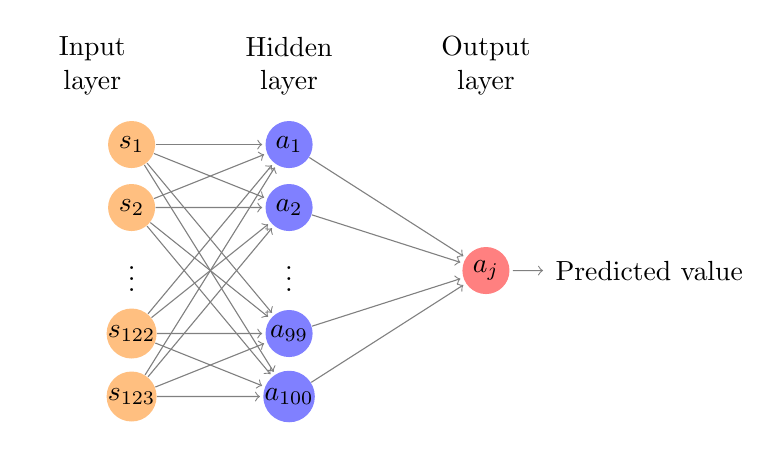
\begin{tikzpicture}[shorten >=1pt,->,draw=black!50, node distance=\layersep, scale=0.8]
    \tikzstyle{every pin edge}=[<-,shorten <=1pt]
    \tikzstyle{neuron}=[circle,fill=black!25,minimum size=17pt,inner sep=0pt]
    \tikzstyle{input neuron}=[neuron, fill=orange!50];
    \tikzstyle{output neuron}=[neuron, fill=red!50];
    \tikzstyle{hidden neuron}=[neuron, fill=blue!50];
    \tikzstyle{annot} = [text width=4em, text centered]

    % Draw the input layer nodes
    \node[input neuron] (I-1) at (0,-1) {$s_1$};
    \node[input neuron] (I-2) at (0,-2) {$s_2$};
    \node at (0,-3) {$\vdots$};
    \node[input neuron] (I-3) at (0,-4) {$s_{122}$};
    \node[input neuron] (I-4) at (0,-5) {$s_{123}$};
    
 
    % Draw the hidden layer nodes
    \node[hidden neuron] (H-1) at (\layersep,-1 cm) {$a_1$};
    \node[hidden neuron] (H-2) at (\layersep,-2 cm) {$a_2$};
    \node (Q-1) at (\layersep,-3 cm) {$\vdots$};
    \node[hidden neuron] (H-3) at (\layersep,-4 cm) {$a_{99}$};
    \node[hidden neuron] (H-4) at (\layersep,-5 cm) {$a_{100}$};

    % Draw the output layer node
    \node[output neuron,pin={[pin edge={->}]right:Predicted value}, right of=Q-1] (O) {$a_j$};

    % Connect every node in the input layer with every node in the
    % hidden layer.
    \foreach \source in {1,...,4}
        \foreach \dest in {1,...,4}
            \path (I-\source) edge (H-\dest);
            
    % Connect every node in the hidden layer with the output layer
    \foreach \source in {1,...,4}
        \path (H-\source) edge (O);

    % Annotate the layers
    \node[annot,above of=H-1, node distance=1cm] (hl) {Hidden layer};
    \node[annot,left of=hl] {Input layer};
    \node[annot,right of=hl] {Output layer};
\end{tikzpicture}
% End of code